%! suppress = NonBreakingSpace
\documentclass[a4paper,12pt]{article}
\usepackage[finnish]{babel}
\usepackage{layout}
\usepackage{graphicx}
\usepackage{geometry}
\usepackage{blindtext}
\usepackage{lastpage}
\usepackage{listings}
\usepackage{multirow}
\usepackage{amsmath}
\usepackage{url}
\usepackage{listings}
\usepackage{listings-rust}
\usepackage{tikz}
\usepackage{setspace}
\usepackage{framed}
\usepackage{parskip}
\usepackage[style=vancouver]{biblatex}
\usepackage{xcolor}
\usepackage{tabularray}
\addbibresource{mendeley.bib}
% \usepackage{showframe}
\lstset{language=Rust, style=boxed,
captionpos=b,
 literate={ö}{{\"o}}1
           {ä}{{\"a}}1
}
\renewcommand{\lstlistingname}{Lähdekoodi}
\interfootnotelinepenalty=10000


\usepackage{tikz}
\usetikzlibrary{positioning,shapes,shadows,arrows}

\tikzstyle{struct}=[rectangle, draw=black, text centered, anchor=north, text=black, text width=4cm]
\tikzstyle{thread}=[rectangle, draw=black, text centered, anchor=north, text=black, text width=4cm]
\tikzstyle{app}=[rectangle, draw=black, text centered, anchor=north, text=black, text width=3cm]



\newcommand{\architecture}{
\begin{figure}[h!]
\centering
    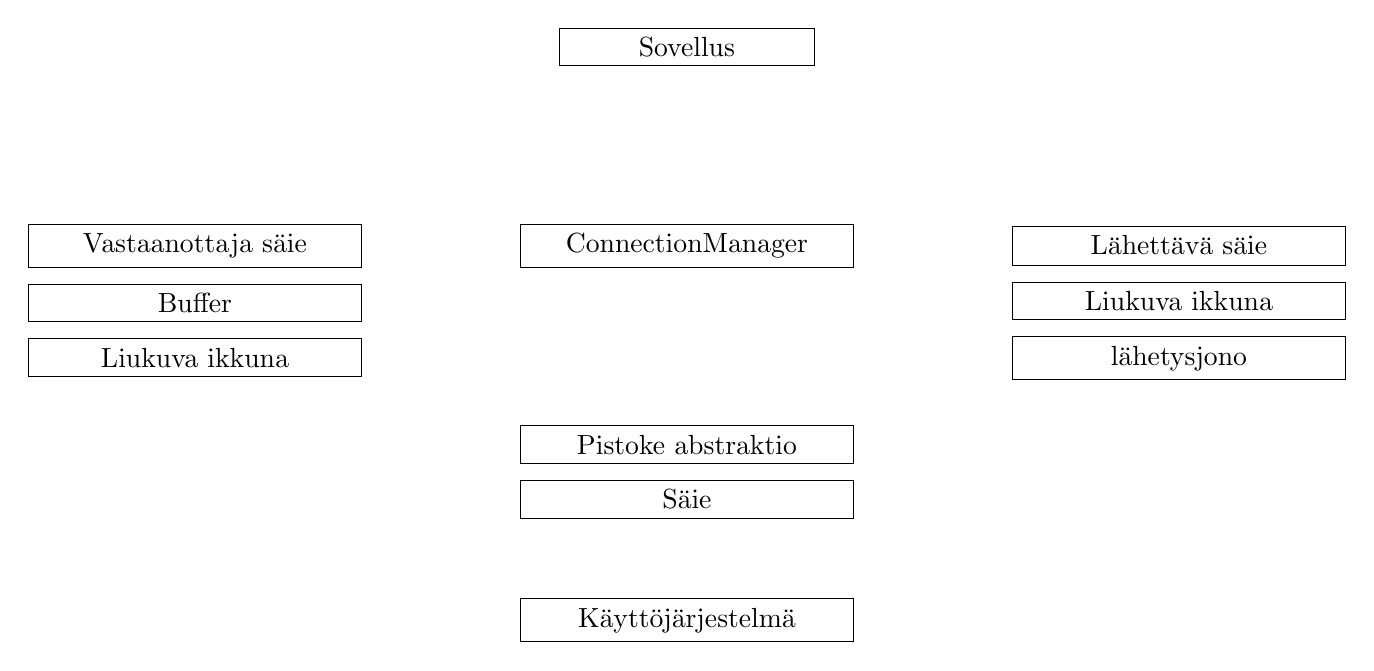
\begin{tikzpicture}[node distance=2cm]
        \node(app)[app]{
            Sovellus
        };
        \node(ConnectionManager)[struct, below=of app] {
            ConnectionManager
        };
       \node(rthread)[thread, left=of ConnectionManager]{
            Vastaanottaja säie
       };
       \node(buffer)[struct, below=0.2cm of rthread] {
            Buffer 
       };
       \node(rwindow)[struct, below=0.2cm of buffer] {
            Liukuva ikkuna 
       };
       \node(tthread)[thread, right=of ConnectionManager]{
            Lähettävä säie
       };
       \node(twindow)[struct, below=0.2cm of tthread] {
            Liukuva ikkuna 
       };
       \node(queue)[struct, below=0.2cm of twindow] {
            lähetysjono
       };
       \node(socket)[struct, below=of ConnectionManager]{
            Pistoke abstraktio
       };
       \node(socketthread)[struct, below=0.2cm of socket]{
            Säie
       };
       \node(os)[struct, below=1cm of socketthread]{
            Käyttöjärjestelmä
       };
    \end{tikzpicture}
    \caption{Arkkitehtuuridiagrammi} \label{fig:arkkitehtuuri}
\end{figure}
}


\onehalfspacing






\title{Luotettava UDP-yhteys}
\author{Joonas Kajava}
\date{\today}

\newcommand{\me}{Joonas Kajava}
\renewcommand{\title}{Luotettava UDP-yhteys}

\newcommand{\appendixCount}{0}

\newcommand{\pageCount}{ \pageref{LastPage}}

\newcommand*\sepline{
    \begin{center}
        \rule[1ex]{\textwidth}{.5pt}
    \end{center}}


\begin{document}
    \begin{titlepage}
        
\includegraphics[width=0.5\textwidth]{images/metropolia}\par\vspace{2cm}
        {\Large \me}\par \vspace{1cm}

        {\Huge \title}\par \vspace{1cm}

        \vfill

        Metropolia Ammattikorkeakoulu\par
        Insinööri (AMK)\par
        Tieto ja viestintätekniikka\par
        Insinöörityö\par
        \today

        \newpage
        \thispagestyle{empty}

        \section*{Tiivistelmä}

        \begin{tabular} {l l}
            Tekijä:               & \me                                            \\
            Otsikko:              & \title                                         \\
            Sivumäärä:            & \pageCount{} sivua + \appendixCount{} liitettä \\
            Aika:                 & \today                                         \\
            \\
            Tutkinto: & Insinööri (AMK) \\
            Tutkinto-ohjelma: & Tieto- ja viestintätekniikka \\
            Ammatillinen pääaine: & Ammatillinen pääaine \\
            Ohjaajat: & Tehtävänimike Etunimi Sukunimi                      \\
            & Tehtävänimike Etunimi Sukunimi \\
        \end{tabular}
        \sepline
        \newpage
        \thispagestyle{empty}


        \tableofcontents
        \newpage
        \thispagestyle{empty}


        \section*{Lyhenteet}
        \begin{tabular}{l l}
            UDP: & User Datagram Protocol        \\
            TCP: & Transmission Control Protocol \\
            IP:  & Internet Protocol             \\
            ACK: & Acknowledgement               \\
            NAK: & Negative Acknowledgement      \\
            NIC: & Network Interface Controller  \\
            ARQ: & Automatic Repeat Request      \\
            IPC: & Inter-Process Communication   \\
        \end{tabular}
        \newpage


    \end{titlepage}


    \section{Johdanto}\label{sec:johdanto}
    Tässä työssä käsitellään teoria internet protokollan luomiseen. Teorian jälkeen lukija ohjataan vaiheittan internet protokollan luomiseen UDP:n päälle. Tämän työn tarkoitus on luoda pohja yrityksille ja kehittäjille, minkälainen on internet protokollan toteutus ja mihin asioihin täytyy ottaa huomiota.
    \par Työ on luonteeltaan tutkivaa ja tarkoitus on luoda selkeä pohja minkä perusteella on yksinkertaista hyödyntää UDP-protokollaa reaaliaikaisiin ohjelmiin.


    \section{Internet-protokollat}
    TCP ja UDP protokollat ovat kaksi yleisintä TCP/IP protokollaa.
    Näistä TCP protokolla on usein käytetty palveluissa, jotka vaativat vakaata ja luotettavaa yhteyttä. UDP paras reaaliaikaisia sovelluksia varten. Tämä johtuu siitä, että TCP paketin mukana liikkuu paljon reservoituja tavuja, joita ei käytetä ollenkaan, myös otsikko päättyy turhaan täytteeseen.
    \par
    UDP:n etu realiaikaisessa kommunikaatiossa on, että se on kevyt ja nopea.
    \cite{KumarSurveyUDP}
    \par



    \section{Tavoitteet ja motivaatio}
    Tämän työn tavoitteena on internet protokollien toimintaa ja niiden implementointia. Tilanteissa missä kaistanleveys on rajallinen ja nopea vasteaika on tärkeää, on usein kannattavaa luoda oma protokolla, joka on räätälöity sovelluksen tarpeita varten.
Oman protokollan käyttöönotto vaatii kohtuullisen määrän tietoa verkkosovittimien, UDP protokollan, yhtäaikaisuudesta sekä tehokkaista tietorakenteista.\par
    Tässä dokumentissa käydään läpi internet protokollien teoriaa, toteutukset käyttäen rust ohjelmointi kieltä ja lopuksi tutkiva osuus jossa mitataan protokollien suorituskykyä ja tehokkuutta.


    \section{Verkkosovitin}\label{sec:verkkosovitin}
    Rust-ohjelmointikieli käyttää linuxissa \textit{libc}-kirjastoa \cite{rust-source-unix-netrs}

    \section{TCP/IP}\label{sec:tcpip}
    \blindtext

    \section{Paketti}\label{sec:paketti}
    Paketti on perustuu TCP:n ja on rakennettu UDP:n päälle. Paketin rakenne on minimaalinen ja yksinkertainen.

\begin{align}
    \text{Frame size} &= F_s \\
    \text{Option size} &= O_s = F_s - F_{min} - D_s
\end{align}



\begin{table}[h!]\
    \centering
    \resizebox{\textwidth}{!}{
        \begin{tabular}{*{33}{|l}|l|}
        \hline
        \multicolumn{2}{|c|}{Offsets} & \multicolumn{8}{|l|}{0}& \multicolumn{8}{|l|}{1}& \multicolumn{8}{|l|}{2}& \multicolumn{8}{|l|}{3} \\ \hline
        Octet & Bit&0&1&2&3&4&5&6&7&0&1&2&3&4&5&6&7&0&1&2&3&4&5&6&7&0&1&2&3&4&5&6&7 \\ \hline
        0 & 0 & \multicolumn{32}{|c|}{Sequence number} \\ \hline
        4&32&RES&RES&RES&RES&RES&RES&EOM&ACK&\multicolumn{8}{|c|}{Reserved}&\multicolumn{8}{|c|}{Data Length}&\multicolumn{8}{|c|}{Data Offset} \\ \hline
        32&64&\multicolumn{32}{|c|}{Options} \\
        ...&...& \multicolumn{32}{|c|}{} \\ \hline
        \multicolumn{2}{|c|}{Data Offset}&\multicolumn{32}{|c|}{Data} \\
        ...&...& \multicolumn{32}{|c|}{} \\ \hline
        \end{tabular}
    }
    \caption{Paketin rakenne}
    \label{tab:my_label}
\end{table}

Tässä työssä paketti on määritelty seuraavasti:
\begin{lstlisting}[caption={Paketin rakenne}, label={lst:frame}]
pub struct Frame {
    frame: [u8; MAX_FRAME_SIZE],
    data_length: usize,
    options_size: usize,
}
\end{lstlisting}
Lähdekoodissa \ref{lst:frame} määritetaan tietorakenne \textit{Frame},
\lstinline{[u8; MAX_FRAME_SIZE]} on taulokkotyyppi joka koostuu tavuista ja on kooltaan yhtä suuri kuin $F_{max}$.
\lstinline{data_length} sisältää tiedon pakettiin tallennetun datan koosta. \lstinline{options_size} sisältää tiedon paketin asetuksien koosta.\par
\lstinline{usize} vastaa kohde arkkitehtuurin muistiosoitteen kokoa. 32 bittisessä kohde tietokoneessa \lstinline{usize} vastaa 4 tavua ja 64 bittisessä kohteessa 8 tavua \cite{rust-doc-usize}.

\subsection{Tietojen käsittely paketissa}
    Paketti on ohjelmanmuistissa yhtenä kokonaisena taulukkona, joka koostuu tavuista.
    Paketti sisältää tietoja 16 bittisessä ja 32 bittisessä muodossa. Nämä tiedot täytyy jakaa tavuihin lähettämistä varten.

\begin{lstlisting}[caption={Järjestusnumeron asettaminen pakettiin}, label={lst:set_seq_num}]
pub fn set_sequence_number(&mut self, sequence_number: u32) {
    let net_sequence_number = sequence_number.to_be_bytes();
    self.frame[SEQUENCE_NUMBER_OCTET..4]
    .copy_from_slice(&net_sequence_number);
}
\end{lstlisting}

Lähdekoodissa \ref{lst:set_seq_num} järjestysnumero muutetaan laskevaan tavujärjestykseen, käyttäen rust standardi kirjaston functiota \lstinline{to_be_bytes()} \cite{rust_doc_u32}. Tämän jälkeen se kopiodaan paketin 4 ensimmäisen tavun tilalle. \par
Oikea tavujärjestys on erittäin tärkeä osa tiedon siirrossa verkon ylitse. Protokollaa käyttävät tietokoneet täytyvät olla yhteisymmärryksessä mitä tavujärjestystä tiedonsiirrossa käytetään. laskeva tavujärjestys on yleisn järjestys, joten päätin käyttää sitä myös tässä protokollassa. \par
Mikäli tavujärjestystä ei ota huomioon tiedonsiirrossa ja vastaanottaja sekä lähettäjän tietokoneet käyttävät eriävää tavujärjestystä, lukujen muuntaminen tavutaulukosta primitiiviseksi luvuksi tuottaa vääriä tuloksia.
\cite{Adiga2007HowC}
// TODO: Lisää jotain diagrameja tähän

    \subsection{Kuljetuskerros}\label{subsec:kuljetuskerros}
    Kuljetuskerros hoitaa pakettien luomisen ja välittämisen paketin verkkosovittimeen.
    Kuljetuskerros määrittelee seuraavat osat protokollasta:

    \begin{itemize}
        \item Paketteihin liittyvät vakiot
        \item Ohjausbitit
        \item Paketin otsakkeen
        \item Paketin lisäasetukset
        \item Vastaanottoikkunan toiminnan
        \item Lähetysikkunan toiminnan
    \end{itemize}

    \subsection{Vakiot}
    Vakiot ovat tärkeitä protokollan toiminnan kannalta. Vastaanottajalla ja lähettäjällä täytyy olla samat vakiot käytössä jotta pakettien muodostaminen sekä lukeminen onnistuu.


    \begin{table}[h!]
        \centering
        \begin{tabular}{llll}
            Vakion-nimi & Lyhenne & Arvo & Yksikkö \\
            \hline
            MAX\_DATA\_SIZE & $D_s$ & 128 & Tavu \\
            SEQ\_NUM\_SIZE & $S_s$ & 4 & Tavu \\
            CONTROL\_BITS\_SIZE & $C_s$ & 1 & Tavu \\
            RESERVED\_SIZE & $R_s$ & 1 & Tavu \\
            DATA\_LENGTH\_SIZE & $DL_s$ & 1 & Tavu \\
            DATA\_OFFSET\_SIZE & $DO_s$ & 1 & Tavu \\
            OPTION\_KIND\_SIZE & $OK_s$ & 1 & Tavu \\
            OPTION\_LENGTH\_SIZE & $OL_s$ & 1 & Tavu \\
            OPTION\_DATA\_SIZE & $OD_s$ & 4 & Tavu \\
            MAX\_OPTION\_COUNT & $MO_c$ & 4 & Määrä
        \end{tabular}
        \caption{Vakiot ja niiden arvot}
        \label{tab:vakiot}
    \end{table}

    Näiden vakioiden perusteella voidaan laskea tärkeitä muuntujia\footnote{Ohjelman kääntäjä laskee nämä ja tallentaa tulokset vakioarvoiksi \cite{rust_book_constant_evaluation}.}.

    \begin{align}
        \text{MIN\_FRAME\_SIZE} &= F_{min} = S_s + C_s + R_s + DL_s + DO_s \\
        \text{MAX\_FRAME\_SIZE} &= F_{max} = F_{min} + MO_c(OK_s + OL_s + OD_s) + D_s \label{eq:fmax}
    \end{align}


    \subsection{Ohjausbitit}\label{subsec:control_bits}
    Ohjausbitit ilmaantuvat paketissa yhtenä tavuna, joista jokainen bitti vastaa tiettyä ohjausbittiä.

    \begin{table}[h!]
        \centering
        \begin{tabular}{lll}
            Nimi & Lyhenne & Binääriarvo \\
            \hline
            Kuittaus & ACK & 00000001 \\
            Pääte & EOM & 00000010 \\
        \end{tabular}
        \caption{Ohjausbitit ja niiden arvot}
        \label{tab:control_bits}
    \end{table}

    Taulukon \ref{tab:control_bits} määrittämät ohjausbitit antavat vastaanottajalle tärkeää tietoa paketista. Kuittausbitti ilmoittaa lähettäjälle, että vastaanottaja on saanut paketin onnistuneesti. Pääte bitti ilmoittaa vastaanottajalle, että kyseinen paketti on paketti ryhmän viimeinen ja ryhmä on valmis koottavaksi kun kaikki sitä edeltävät paketit ovat saapuneet. \par
    Vastaanottaja tarkistaa ohjausbittien olemassaolon bittioperaatiolla.
\begin{lstlisting}[caption={Kuittasbitin tarkistus ohjausbiteistä}, label={lst:ack_check}]
if control_bits & 00000001 == 00000001 {
    // Kuittausbitti löytyy
}
\end{lstlisting}




    \subsection{Sovelluskerros}\label{subsec:sovelluskerros}
    \blindtext


    \section{UDP}\label{sec:udp}
    \blindtext


    \section{Arkkitehtuuri}\label{sec:arkkitehtuuri} 
    \architecture

     \lstinline{ConnectionManager} on vastuussa yhteyksien hallinnasta. Sen tehtävä on 
    hoitaa vastaanottaja säiettä ja lähettävää säiettä. Kun sovellus haluaa käynnistää yhteyden, 
    \lstinline{ConnectionManager} luo pistokkeen sovelluksen antamaan osoitteeseen. 
    Lähetys ja vastaanotto säikeet käynnistyvät kun pistokkeen luonti onnistuu. 
    \par
    \begin{lstlisting}[caption={ConnectionManager rakenne}, label={lst:connectionmanager}]
pub struct ConnectionManager {
    listener_thread: Option<thread::JoinHandle<()>>,
    transmitter_thread: Option<thread::JoinHandle<()>>,
    socket: Arc<SocketAbstraction>,
    message_sender: SyncSender<Vec<u8>>,
}\end{lstlisting}

\begin{lstlisting}[caption={Drop ominaisuuden toteutus ConnectionManager:ille}, label={lst:connectionmanager_drop}]
impl Drop for ConnectionManager {
    fn drop(&mut self) {
        if let Some(x) = self.listener_thread.take() {
            x.join().unwrap();
        }
        if let Some(x) = self.transmitter_thread.take() {
            x.join().unwrap();
        }
    }
}
\end{lstlisting}


    \lstinline{ConnectionManager} pitää muistissa viitteet vastaanottaja ja lähettäjä säikeisiin.
    \lstinline{Option<...>} määrittelee valinnaisen arvon, joka tarkoittaa, että kyseinen muuntuja ei 
    välttämättä sisällä käyttökelpoista arvoa. Tämä vastaa muissa useissa ohjelmointikielissä \lstinline{null} arvoa \cite{rust_book_enum}. Näitä kahta muuntujaa käytetään säikeiden sulavaan sulkemiseen kun \lstinline{ConnectionManager} pudotetaan muistista. 

    \lstinline{ConnectionManager} implementoi \lstinline{Drop} ominaisuuden, joka liittää vastaanottaja
    ja lähettäjä säikeet. Näin ohjelma jää odottamaan, että nämä kaksi säiettä sulkeuduu oikein \cite{rust_doc_joinhandle}.
        
    \section{Liukuva ikkuna}\label{sec:liukuva_ikkuna}
    \begin{lstlisting}[caption={Ikkunan rakenne}, label={lst:window}]
pub struct Window {
    frame_status: Vec<bool>,
    window_size: u32,
    window_left_edge: u32,
}\end{lstlisting}


    \begin{lstlisting}[caption={Vastaanottajan ikkunan rakenne}, label={lst:rwindow}]
pub struct ReceiverWindow {
    inner_window: Window,
    buffer: Vec<Option<Frame>>,
}\end{lstlisting}

    \begin{lstlisting}[caption={Lähettävän ikkunan rakenne}, label={lst:twindow}]
pub struct TransmitterWindow {
    inner_window: Window,
    socket: Arc<SocketAbstraction>,
    events_sender: Sender<ConnectionEventType>,
    ack_receiver: Receiver<u32>,
    data_queue: Vec<Option<QueueFrame>>,
}\end{lstlisting}

Tässä ohjelmassa puskurit ovat toteutettu käyttämällä heap allokoituja vektoreita. \lstinline{Vec} on yleisesti paras tietorakenne tämän tyylisiä operaatioita varten. Vertailu muihin tietorakenteisiin löysyy osiosta \ref{sec:suorityskyky}.

    \subsection{Ikkunan siirto vastaanottaessa}

    \begin{align}
        n_s &= \text{Pienin vastaanotettu järjestysnumero} \\
        n_x &= \text{Vastaanotetun paketin järjestysnumero} \\
        w_s &= \text{Ikkunan koko}
    \end{align}



Vastaanottajan ikkuna määritellään lähdekoodin \ref{lst:rwindow} mukaisesti. Se sisältää yleisen \lstinline{Window} toteutuksen ja \lstinline{buffer} kentän, jonka tarkoitus on pitää tietoja 
tallessa ennenkuin ne kasataan yhdeksi kokonaisuudeksi. \par
Rust-kielessä ei pysty tekemään perintää samantyylisesti kuin yleisissä OOP-kielissä. Tämän takia
käytetään suunnittelutapaa nimeltä "\textit{Composition over Inheritance}" \cite{Ivicevic202228Inheritance}.

\begin{framed}
    Vastaanottava ikkuna pitää muistissa pienimmän järjestysnumeron $n_s$, minkä se on vastaanottanut. 
Vastaanottava ikkuna hylkää kaikki paketit, joiden järjestysnumero on ikkunan ulkopuolella $n_x < n_s$ tai $n_x > n_s + w_s$. Jos järjestysnumero on ikkunan sisällä, se hyväksytään ja merkitään vastaanotetuksi. Mikäli $n_x = n_s + 1$ ikkunaa voidaan siirtää eteenpäin.
    Ikkunan siirto tapahtuu kulkemalla hyväksyttyjen järjestysnumeroiden listaa eteenpäin, kunnes vastaan tulee järjestysnumero jota ei ole vielä vastaanotettu. Kulkiessa tapahtuneiden askelien määrä lisätään muuntujaan $n_s$.
\end{framed}

    Tässä toteutuksessa $n_s$ löytyy yleisen ikkunan (lähdekoodi \ref{lst:window}) sisältä kentästä \lstinline{window_left_edge: u32}.
    

    \section{Vastaanottajan toiminta}
    Datan vastaanottaminen tapahtuu vastaanottaja säikeessä, joka käynnisttään yhteyden muodostamisessa.
    Säie pyörii ikuisessa silmukassa, jossa ensimmäinen operaatio on ikkunan siirto eteenpäin.

\begin{lstlisting}[caption={Ikkunan siirto}, label={lst:shift_window}]
pub fn shift_window(&mut self) -> usize {
    let mut shift_amount = 0usize;
    for e in self.frame_status.iter() {
        if *e {
            shift_amount += 1;
        } else {
            break;
        }
    }
    self.frame_status.drain(0..shift_amount);
    self.window_left_edge += shift_amount as u32;
    shift_amount
}
\end{lstlisting}      

Lähdekoodi \ref{lst:shift_window} esittää yleisen ikkunan siirtämistä eteenpäin.
\lstinline{self.frame_status} viittaa onnistuneesti lähetettyihin tai vastaanotettuihin paketteihin.


\begin{lstlisting}[caption={Vastaanottajan ikkunan siirto}, label={lst:shift_rwindow}]
pub fn shift_window(&mut self) -> Vec<Frame> {
    let shift_amount = self.inner_window.shift_window();
    let shifted_frames = self.buffer.drain(0..shift_amount);
    let result = shifted_frames.into_iter().flatten().collect();
    self.buffer.shrink_to_fit();
    result
}
\end{lstlisting}

Sisäisen ikkunan siirron jälkeen puskuria siirretään eteenpäin. Tämä operaatio tuottaa 
listan paketeista jotka ovat saapuneet onnistuneesti ja ovat oikeassa järjestyksessä.
lista käsitellään \lstinline{flatten()} functiolla joka tuottaa listan missä \lstinline{Option} 
on suodatettu pois. Lopuksi puskurin kapasiteettia kutisteaan\footnote{Tämä operaatio on 
turhan raskas tässä tilanteessa, mutta tähän palataan myöhemmin suorituskyky osiossa.
}. Käsitelty lista palautetaan ja se siirtyy käsiteltäväksi ylempiin kerroksiin. \par

Ylemmässä kerroksessa tämä käsitelty lista käydään läpi.  

\begin{lstlisting}[caption={Pakettien käsittely}, label={lst:handle_shift_window}]
receiving_window.shift_window().into_iter().for_each(|frame| {
    buffer.extend_from_slice(frame.get_data());
    let control_bits = ControlBits::from_bits(frame.get_control_bits())
        .unwrap();
    connection_events_sender_receiver
        .send(ConnectionEventType::ReceivedFrame(frame))
        .unwrap();
    if control_bits.contains(ControlBits::EOM) {
        let message: Vec<u8> = std::mem::take(&mut buffer);
        connection_events_sender_receiver
            .send(ConnectionEventType::ReceivedCompleteMessage(message))
            .unwrap();
    }
});
\end{lstlisting}

Jokainen valmis paketti käydään läpi ja sen sisältö lisätään puskuriin\footnote{Tässä toteutuksessa putkuri on sovelluksen muistissa, mutta isojen viestien siirrossa voidaan myös käyttää tiedostoja puskurina.}
. Tämän jälkeen ohjausbitit luetaan paketista kappaleen \ref{subsec:control_bits} mukaisesti. Ylempiin kerroksiin lähetetään tieto vastaanotetusta paketista käyttäen kanavia, ylemmät kerrokset kuten sovellus voivat käyttää tätä tietoa esim. lataus indikaattorin tekemisessä. \par

Mikäli paketti on viimeinen viesti, puskuri siirretään uuteen listaan ja lähetetään ylemmille kerroksille.



    \subsection{Valikoiva toisto ARQ}\label{subsec:valikoiva_toisto}
    Valikoida toisto ARQ englanniksi \textit{Selective Repeat} on tehokkaampi verrattuna toisiin ARQ protokolliin. 

    \begin{framed}
       \textit{Stop-and-wait ARQ} lähettäjä jää odottamaan jokaisesta paketista kuittausta ennen siirtymistä seuraavan paketin lähettämistä. Vastaavasti vastaanottaja hylkää kaikki paketit jotka eivät ole seuraava paketti järjestyslukujen perusteella \cite{StopAndWaitARQ}. 
    \end{framed}

    Tässä toteutuksessa käytetään valikoivaa toistoa, sillä se on tehokas tiedonsiirron kannalta, mutta se vaatii vastaanottajalta datan puskuroinnin. Puskurointi vaatii huomattavaa muistin\footnote{Tämä toteutus voi vaatia vastaanottajan tietokoneelta noin 2 gigatavua muistia} käyttöä jota ei mahdollisesti ole pienissä laitteissa. Tämä toteutus on tehty sillä oletuksella, että alustana on tietokone ja muistista ei ole pulaa.\par 

    Valikoivassa toistossa lähettäjä lähettää kaikki ikkunan sisällä olevat paketit ja odottaa vastaanottajan kuittauksia. Mikäli lähettäjä vastaanottaa kuittauksia ikkunan etupäästä, lähettäjä siirtää ikkunaa eteenpäin ja lähettää paketit jotka ovat nyt ikkunan sisällä. Tämä jatkuu niin kauan kuin kaikki paketit on lähetetty puskurista. \par 

    Vastaanottaja vastaanottaa kaikki paketit joiden järjestysnumero on ikkunan sisällä vaikka ne tulisi perille väärässä järjestyksessä. Pakettien data tallennetaan puskuriin järjestysnumeron määrittämään indeksiin. Mikäli vastaanottaja vastaanottaa paketteja jotka ovat ikkunan etupäässä, ne siirretään ylemmille kerroksille käsiteltäväksi ja ikkunaa siirretään eteenpäin.    

\section{Viestien käsittely}
Protokolla käsittee vain binääridatan lähettämistä. Monimutkaisien tietorakenteiden kuten objektien lähettäminen protokollan kautta täytyy tehdä binäärikoodauksen kautta. Verkkosivustoissa käytetään usein tekstipohjaisia tietomuotoja, kuten HTML ja JSON. Nämä tietomuodot eivät sovellu reaaliaikaiseen kommunikaatioon, sillä niiden mukana tulee ylimääräisiä merkkejä, joita käytetään skeeman välitykseen. Spesialisoidut reaaliaikaiset sovellukset eivät tarvitse skeematietoja tiedon lukemiseen, sillä osapuolien välillä liikkuva tieto on todella tarkkaan määritelty\footnote{Tämä ei kuitenkaan rajoita sovellusta käyttämään yksinkertaisia rakenteita. Halutessaan sovellus pystyy käyttämään tietorakennetta, joka sisältää skeematietoja.}. \par
\subsection{Skeemapohjainen tieto}
Skeemapohjaista dataa kannattaa hyödyntää silloin, kun vastaanottajalla ei ole tietossa tietoa siitä, miten dataa täytyy lukea. Tästä hyvä esimerkki on konfiguraatio data.
Useat konfiguraatio mahdollisuudet eivät ole pakollisia ja sen takia niille on määritelty oletusarvot. Konfiguraatio voi sisältää tuhansia eri vaihtoehtoja ja ne ovat nimetty tietynlailla. \par
Mikäli tätä konfiguraatiota haluttaisiin muuttaa verkon yli tulevalla tiedolla, skeemapohjainen data soveltuu tähän parhaiten. Näin lähettäjä pystyy kertomaan viestissä, miten dataa luetaan.

\begin{lstlisting}[caption={JSON data}, label={lst:json_data}]
{
    "name": "Joonas Kajava"
}
\end{lstlisting}

    \begin{table}[h!]
        \centering
        \begin{tblr}{
        colspec = {lllll},
        cell{1}{1} = {cyan},
        cell{1}{2-5} = {teal},
        cell{2}{1} = {purple},
        cell{2}{2-5} = {pink},
        row{3-4} = {pink}
        }
00000100&01101110&01100001&01101101&01100101\\
00001101&01001010&01101111&01101111&01101110\\
01100001&01110011&00100000&01001011&01100001\\
01101010&01100001&01110110&01100001\\
        \end{tblr}
        \caption{Binääridata, joka sisältää saman tiedon kuin \ref{lst:json_data} lähdekoodissa}
        \label{tab:binary_data}
    \end{table}

Lähdekoodissa \ref{lst:json_data} ja taulokossa \ref{tab:binary_data} havainnollistetaan kaksi tapaa koodata data tiedonsiirtoa varten. JSON data on helposti luettavaa, mutta se sisältää ylimääräisiä merkkejä, joita tietokone ei tarvitse. Binääritieto sisältää kaiken tarvittavan tiedon, joka riittää tietokoneelle, mutta tekee siitä vaikeasti luettavaa ihmiselle. Binääritieto vie huomattavasti vähemmän tilaa kuin tavallinen JSON data.
Lähdekoodin \ref{lst:json_data} vie 26 tavua, kun taas taulukon \ref{tab:binary_data} vie 19 tavua. Tämän eron huomattavuus suurenee, kun tieton määrä kasvaa. \par

Tässä toteutuksessa on käytetty \lstinline{bincode}\footnote{Saatavilla osoitteesta: https://crates.io/crates/bincode} nimistä kirjastoa binääridatan muodostukseen.

\subsection{Ennalta määritelty data}
Reaaliaikasissa sovelluksissa pitäisi aina pyrkiä siirtämään tietoa ennalta määritetyssä muodossa, jotta voidaan välttää ylimääräisen tiedon välittämisen verkon yli. 


    \begin{table}[h!]
        \centering
        \begin{tblr}{
        colspec = {llll},
        cell{1}{1} = {cyan},
        cell{1}{2-5} = {teal},
        }
        00000001&00000010&00000011&00000100 \\
        \end{tblr}
        \caption{Pelaajan sijainti binääritietona}
        \label{tab:binary_data_player}
    \end{table}

    Tässä toteutuksessa on käytetty binääridata muotoa, jossa ensimmäinen tavu kertoo tiedon muodon. Onkoon tämä ensimmäinen tavu nimeltään jatkossa \textit{"toimintotieto"} Taulukossa \ref{tab:binary_data_player} esimerkki pelaajan sijainnista binäärimuodossa. \par

    Vastaanottaja lukee viestisä ensimmäisen tavun ja sen perusteella valitsee oikean strategian tiedon käsittelyyn. Tässä toteutuksessa toimintotieto on yksi tavu, joka sallii 255 eri toimintoa. Mikäli tämä ei riitä, voidaan käyttää yhtä toimintoa skeemadatan siirtämiseen, jonka käytännössä avaa mahdollisuuden käyttää loputtoman määrän toimintoja. Toinen vaihtoehto suurentaa toimintotietoa kahteen tavuun tai neljään. \par

    Demossa, josta puhutaan myöhemmin kappaleessa \ref{sec:demo}, käytetään neljää toimintoa:
    \begin{enumerate}
        \item String
        \item FileInfo
        \item ResponseToFileInfo
        \item FileData
    \end{enumerate}

    \section{Virheenkorjaus}\label{sec:virheenkorjaus}
    Saapuneiden tietojen varmistukseen käytetään tarkistussummaa. Saapuneen paketin sisällöstä muodostetaan deterministinen luku, jota verrataan paketin mukana tulleeseen tarkistussumman. Mikäli summat eivät vastaa toisiaan voidaan olettaa, että paketti on korruptoitunut ja vastaanottaja lähettää \textit{NACK}-paketin. Kyseinen paketti vaatii lähettäjää lähettämään korruptoituneen paketin uudestaan
    \cite{khan-udp}.
    \subsection{Tarkistussumma}
    
    \begin{table}[h!]
        \centering
        \begin{tblr}{
        colspec = {llllllll},
        cell{7}{3-4} = {purple7},
        cell{7}{5-8} = {lime},
        row{8-9} = {lime},
        }
            18&00&00&00&60&03&82&28 \\
            00&1c&11&80&00&00&00&00 \\  
            00&00&00&00&00&00&00&00 \\
            00&00&00&01&00&00&00&00 \\
            00&00&00&00&00&00&00&00 \\
            00&00&00&01&30&39&30&39 \\ 
            00&1c&c2&a7&00&00&00&01 \\ 
            02&00&0c&08&00&68&65&6c \\
            6c&6f&20&77&6f&72&6c&64 \\
        \end{tblr}
        \caption{UDP-paketti Hex-muodossa, jossa tarkistussumma merkitty purppuralla ja vastaavasti data vihreällä.}
        \label{tab:hello-world}
    \end{table}

    UDP-paketissa tarkistussumma koostuu kahdesta tavusta. Se esiintyy paketin rakenteessa juuri ennen dataa. Taulukko \ref{tab:hello-world} havainnollistaa tarkistustumman(purppura) ja datan(virheä) sijainnin paketissa.

\begin{minipage}{\linewidth}
\begin{lstlisting}[caption={Tarkistussumman muodostaminen}, label={lst:creating_checksum}]
fn calculate_checksum(data: &[u8]) -> u16 {
    let mut sum = 0u32;
    for pair in data.chunks(2) {
        let mut checksum = 0u16;
        checksum += u16::from(pair[0]) << 8;
        checksum += u16::from(pair.get(1).cloned()
        .unwrap_or_default());
        sum += checksum as u32;
    }
    while sum > 0xffff {
        let carry = sum >> 16;
        sum &= 0xffff;
        sum += carry;
    }
    !sum as u16
}
\end{lstlisting}
\end{minipage}

Lähdekoodissa \ref{lst:creating_checksum} muodostetaan 16-bittinen tarkistussumma. 
\lstinline{data}-taulukon sisältämät tavut ryhmitetään 16-bittisiksi numeroiksi, jonka jälkeen ne summataan yhteen. Vaikka lopullinen tarkistussumma täytyy olla 16-bittinen, lukujen summa tallenne taan väliaikaisesti 32-bittiseen numeroon. Tämä täytyy tehdä sen takia, jotta summa operaatiossa ei tapahdu ylivuotoa. Ilman 32-bittisen numeron apua olisi mahdollista, että summa numero ylivuotaa kun se ylittää $2^{16} - 1$ summan
\cite{udp-calculation}.


\begin{framed}
    C-ohjelmointikielessä kokonaisluvun ylivuotoa ei ole määritelty. Tämä voi ja on johtanut useisiin tietoturva ongelmiin. Se saattaa olla usein myös vaikeita löytää sillä C-ohjelma jatkaa toimintaa vaikka ylivuoto tapahtuu.\par
    Rust-ohjelmointikielessä kokonaisluvun ylivuoto on määritelty. Ylivuoto johtaa aina ohjelman paniikkiin ja sitä myötä sen sammumiseen. Tämä käytännössä eliminoi ylivuodon aiheuttamat tietoturva ongelmat \cite[ch.~3.2]{rust-book}.
\end{framed}

\begin{minipage}{\linewidth}

\begin{lstlisting}[caption={Tietojen kasaaminen tarkistussummaa varten}, label={lst:data_for_checksum}]
#[test]
fn checksum() {
    let ip = 1u128.to_be_bytes();
    let port = 12345u16.to_be_bytes();
    let protocol = 0x0011u32.to_be_bytes();
    let payload = [
        0x00, 0x00, 0x00, 0x01, 
        0x02, 0x00, 0x0c, 0x08, 
        0x00, 0x68, 0x65, 0x6c, 
        0x6c, 0x6f, 0x20, 0x77, 
        0x6f, 0x72, 0x6c, 0x64,
    ];
    let udp_packet_length = 28u16;
    let udp_packet_length = udp_packet_length.to_be_bytes();
    let mut data = vec![];
    data.extend_from_slice(&ip);
    data.extend_from_slice(&ip);
    data.extend_from_slice(&protocol);
    data.extend_from_slice(&udp_packet_length);
    data.extend_from_slice(&port);
    data.extend_from_slice(&port);
    data.extend_from_slice(&udp_packet_length);
    data.extend_from_slice(&payload);
    let checksum = calculate_checksum(&data);
    assert_eq!(checksum, 0xc2a7);
}
\end{lstlisting}
\end{minipage}

Lähdekoodissa \ref{lst:data_for_checksum} näytetään miten \lstinline{data: &[u8]} muodostetaan. Tarkistussumma sisältää lähettäjän ja vastaanottajan IP-osoitteet, portit, protokolla (17), UDP-osuuden koon ja lopuksi kuorman \cite{RFC-768, protocol-numbers}. \par
    
    Modernien tietokoneiden verkkokortti hoitaa tämän tarkistussumman käsittelyn \cite{TCP/IPLearn}. 

    \section{Demo}\label{sec:demo}

    \begin{figure}[h!]
        \centering
        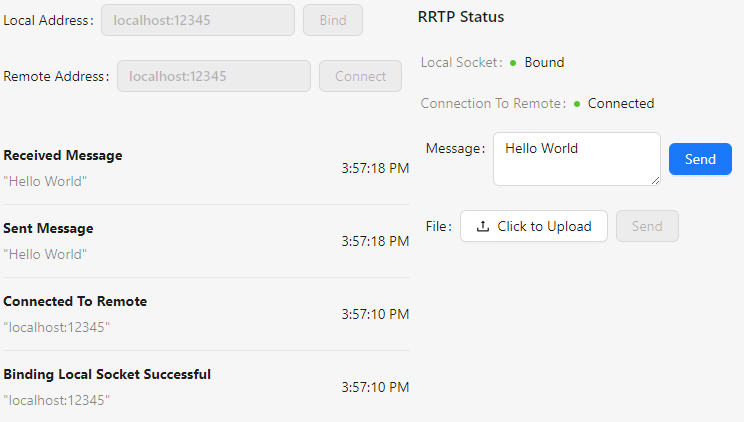
\includegraphics[width=\textwidth]{doc/latex/src/images/RRTP.png}
        \caption{Demo-ohjelman käyttöliittymä}
        \label{fig:demo_interface}
    \end{figure}
    
    Iso osa tätä työtä oli myös toteuttaa esimerkki ohjelma jolla pystyy luotettavasti siirtää tiedostoja ja viestejä verkon yli. Demo-sovellus on rakennettu käyttäen Tauri- ja React-kirjastoa. Koska Rust-ohjelmointikieli on vielä nuori, käyttöliittymä ekosysteemi ei ole vielä kypsä \cite{AreYet}. Tämän takia päädyin Tauri-kirjastoon, joka hyödyntää webteknologioita käyttöliittymän piirtämiseen ja ohjaamiseen. Taustalla pyörii Rust-ohjelma joka hoitaa tiedon siirron. \par
    Egui\footnote{Egui on kypsä ja sillä on hyvä dokumentaatio, mutta \textit{immidiate mode} aiheutaa vaikeuksia ulkoasun määrittelyssä. } ja Iced projektit olivat hyviä vaihtoehtoja, mutta dokumentaatio ja yleinen kypsyys ei ollut riittävä tämän projektin tilanteeseen. \par


    Demo-sovellus on rakennettu käyttäen Tauri-ohjelmistokehystä.
    Tauri on electronin kaltainen ohjelmistokehys \footnote{Electron pyörii Node.js runtime ympäristön päällä ja tarjoaa version Chromium selaimesta käyttöliittymän piirtämiseen.}, joka mahdollistaa sovelluksien rakentamisen käyttäen web-teknologioita. Taustalla pyörii Rust-prosessi, joka luo ikkunan käyttäen \textit{TAO}-ohjelmistokirjastoa. Tämän jälkeen \textit{WRY}-ohjelmistokirjasto luo \lstinline{WebView} elementin, joka kutsuu käyttöjärjestelmän tarjoamaa selainta näyttämään sivuston \cite{tauri-app}.

    Demo-ohjelmasta löytyy kaksi kenttää osoitteiden asettamiseen. Lista, joka 
    pitää kirjaa tapahtumista. Tilannepaneeli, joka näyttää yhteyden tilan. 
    Kaksi kenttää viestien ja tiedostojen lähettämiseen. \par

    \subsection{Riippuvuudet}
    Demo-sovelluksessa on mahdollista käyttää \textit{crates.io}-palvelun\footnote{Saatavilla osoitteesta: https://crates.io/} rust-paketteja ja \textit{npm}-palvelun\footnote{Saatavilla osoitteesta: https://www.npmjs.com/} javascript-paketteja. Paketit sallivat nopean kehityksen ja tarjoavat vakaita ratkaisuja eri ongelmiin. Usein pakettien käyttäminen on erittäin suositeltua, sillä niiden dokumentaatio ja valmiit ratkaisut ovat hyödyksi kehityksessä ja ylläpitämisessä.
    
    \begin{table}[h!]
        \centering
        \begin{tblr}{
        colspec = {lll},
        row{even} = {lightgray},
        }
        Nimi&Käyttötarkoitus \\
        \hline
        tauri & Käyttöliittymän piirtäminen \\
        serde/bincode & Tiedon serialisointi ja deserialisointi \\
        fern/log/humantime & Lokitiedostojen kirjoittaminen \\
        typeshare & Typescript-rajapintojen luonti automaattisesti Rust-tyypeistä \\
        infer & Tiedostotietojen lukeminen \\
        thiserror/anyhow & Virheilmoituksien luonti ja käsittely 
        \end{tblr}
        \caption{Rust-riippuvuudet}
        \label{tab:cargo_dependencies}
    \end{table}

    
    \begin{table}[h!]
        \centering
        \begin{tblr}{
        colspec = {lll},
        row{even} = {lightgray},
        }
        Nimi&Käyttötarkoitus \\
        \hline
        ahooks & Hyödyllisiä React-koukkuja \\
        antd & Käyttöliittymä-elementit \\
        dayjs & Aika-tietojen käsittely \\
        pretty-bytes & Tiedostokoon muuntaminen ihmisluettavaksi \\
        rc-virtual-list & Virtuaaliset listat \\
        react/react-dom & Käyttöliittymän hallinta ja piirtäminen \\
        recoil & Käyttöliittymän tilan hallinta \\
        typescript & Tyyppitietojen lisääminen javascriptiin \\
        vite & Front-end ohjelmiston prosessointi
        \end{tblr}
        \caption{npm-riippuvuudet}
        \label{tab:npm_dependencies}
    \end{table}

    \subsection{Ohjelman käynnistysvaihe}

    Demo-ohjelma alkaa \lstinline{main.rs}-tiedoston \lstinline{fn main()}-funktiosta. 
    Se suorittaa 5 tärkeää toimintoa: lokituskonfiguraatio, sovellustilan alustaminen, lokiseurant säikeen käynnistys, IPC-rajapintojen määritys ja lopuksi käyttöliittymän käynnistys. \\

    \begin{lstlisting}[caption={Lokituskonfiguraatio}, label={lst:logging_config}]
fern::Dispatch::new()
.format(|out, message, record| {
    out.finish(format_args!(
        "[{} {} {}] {}",
        humantime::format_rfc3339_seconds(SystemTime::now()),
        record.level(),
        record.target(),
        message
    ))
})
.level(log::LevelFilter::Debug)
.chain(std::io::stdout())
.apply()?;
    \end{lstlisting} 

    \begin{lstlisting}[caption={Esimerkki lokitapahtumasta}, label={lst:log_example}]
[2024-03-29T13:57:18Z INFO messanger::connection_processor]
Processing connection event:
ReceivedCompleteMessage([0, 72, 101, 108, 108, 111, 
32, 87, 111, 114, 108, 100])
    \end{lstlisting}
    

    Lokituskonfiguraatio tapahtuu \lstinline{setup_logger()}-funktion kautta. 
    Lokitus formaatti on asetettu niin, että viestissä ilmenee selkeästi tapahtuma aika,
    viestin taso, tapahtuman moduuli ja itse viestin sisältö. Lähdekoodi \ref{lst:log_example} esittää mahdollisen lokitapahtuman. Sovellus voi kirjoittaa loki tapahtuman käyttämällä \lstinline{log}-kirjaston tarjoamia makroja\footnote{Mahdolliset makrot ovat: debug, error, info, log, trace, warn.}: \lstinline|info!("Processing connection event: {:?}", event);|\par


    
    \begin{lstlisting}[caption={Setup-funktion tunniste}, label={lst:setup_signature}]
pub fn setup<F>(mut self, setup: F) -> Self
where
F: FnOnce(&mut App<R>) -> 
Result<(), Box<dyn std::error::Error>> + Send + 'static
\end{lstlisting}
    



    Sovellustila alustetaan \lstinline{tauri:app:Builder} struktuurin \lstinline{setup}-funktiolla, jonka tunniste on kuvattu lähdekoodissa \ref{lst:setup_signature}. Tämän tunnisteen ymmärtäminen on tärkeää sillä Rust-kääntäjä on erittäin tarkka rajoituksista, mitä tunniste asettaa. Rajoitukset ovat tärkeitä sillä niiden avulla pystytään takaamaan muistiturvallisuus, jopa useiden säikeiden välillä \cite[ch. 8.2]{rust-book}. \par

    Lähdekoodin \ref{lst:setup_signature} tunniste on suhteellisen monimutkainen, mutta se voidaan lukea seuraavasti:
    
    \begin{enumerate}
        \item \lstinline{pub fn} Kyseessä on julkinen funktio \lstinline{setup}.
        \item \lstinline{<F>} on geneerinen tyyppi parametri \lstinline{F}.
        \item \lstinline{mut self} funktio suoritetaan \lstinline{tauri:app:Builder} rakenteella.
        \item \lstinline{setup: F} funktio ottaa vastaan parametrin, jonka tyyppi on geneerisen parametrin \lstinline{F} mukainen.
        \item \lstinline{-> Self} funktio palauttaa \lstinline{tauri:app:Builder} rakenteen.
       \item \lstinline{where} määrittelee geneeriset tyyppi parametrit.
       \item \lstinline{F:} aloittaa \lstinline{F} parametrin määrityksen.
       \item \lstinline{FnOnce(&mut App<R>) ->} määrittelee sulkeuman, joka voidaan suorittaa vähintään kerran. Sulkeuma saa parametrin mukana muuttuvan viitteen \lstinline{App<R>} muuntujaan.
       \item \lstinline{Result<(), Box<dyn std::error::Error>>} tarkoittaa, että sulkeuma ei palauta mitään \lstinline{()} tai se palauttaa virheen joka implementoi \lstinline{std::error::Error} ominaisuuden.
       \item \lstinline{Send} on erittäin tärkeä tieto sulkeumasta. Tämä tarkoittaa sitä, että sulkeuma ja sen käyttämät asiat täytyvät olla turvallisia säikeiden välistä siirtoa varten. Tämä tarkoittaa myös sitä, että demo-sovelluksen tila rakenne on turvallista siirtää toiseen säikeeseen.
       \item \lstinline{'static} on käyttöikätunniste, joka vaatii että sulkeuma ja sen käyttämät asiat ovat koko soveluksen elinajan käyttökelpoisia.
    \end{enumerate}
    \section{Suorityskyky}\label{sec:suorityskyky}

    \subsection{Lista tietorakenteet}
    Tämän ohjelman luonteen kannalta on tärkeää, että käytetään tehokkaita tietorakenteita. Ohjelman täytyy pystyä tehokkaasti käsittelemään listoja jotka sisältävät tuhansia elementtejä. Suorituskyvy testaamisen tuloksien perusteella päädyin \lstinline{Vec} tietorakenteeseen.

    
    Suorituskyvyn mittaaminen toteutetaan sisäverkossa, jotta tiedonsiirto nopeus on deterministinen ja vakaa.
    Testiympäristö koostuu yhdestä Windows tietokoneesta, joka muodostaa yhteyden itseensä käyttäen silmukka osoitetta.\par
    Testissä tietokone siirtää itselleen silmukan kautta 50 megatavun tiedoston. Testi suoritetaan 10 putkeen jotta saadaan leville keskiarvo selville.

    \subsection{Asynkroninen}


    \newpage
    \printbibliography
\end{document}